\documentclass[final,hyperref={pdfpagelabels=false}]{beamer}
\mode<presentation>
{
  % \usetheme{Berlin}
  \usetheme{Prog}
}
\usepackage{times}
\usepackage{amsmath,amsthm, amssymb, latexsym}
\boldmath
\usepackage[english]{babel}
\usepackage[latin1]{inputenc}
\usepackage[orientation=landscape,size=a1,scale=1.4,debug]{beamerposter}
\usepackage{listings}
\usepackage{tikz}
\usetikzlibrary{trees}


%%%%%%%%%%%%%%%%%%%%%%%%%%%%%%%%%%%%%%%%%%%%%%%%%%%%%%%%%%%%%%%%%%%%%%%%%%%%%%%%% 5
\graphicspath{{figures/}}
\title[Fancy Posters]{Supporting Visual Impaired Learners in Editing
  Mathematics}

\author[Volker Sorge]{Volker Sorge}
\institute[U. of Birmingham\& Progressive Access]{Scientific Document Analysis Group, University of Birmingham, UK\\
  Progressive Accessibility Solutions, Ltd, UK\\
\textcolor{orange}{Thanks to TV Raman for his technical work on the Emacspeak
integration.}}
\date{25th October, 2016}


%%%%%%%%%%%%%%%%%%%%%%%%%%%%%%%%%%%%%%%%%%%%%%%%%%%%%%%%%%%%%%%%%%%%%%%%%%%%%%%%% 5
\begin{document}
\begin{frame}{} 
  \vfill
  \begin{columns}[t]
    \begin{column}{.48\linewidth}
      \begin{block}{\Large Motivation}
        \begin{itemize}
        \item Mathematics is the single most significant hurdle for inclusive
          education for visually impaired students in the STEM subjects.
        \item  In secondary
          education increasing complexity of mathematical formulas makes it harder to
          communicate content equally effectively to both sighted and blind students.
        \item Dedicated Braille formats become quickly unwieldy for more
          advanced mathematics
        \item It becomes impossible for students to communicate them to their
          peers or professors.
        \item On Transitioning from high school to University students often
          have to learn {\LaTeX} to have a means to read and communicate
          advanced material.
        \end{itemize}
      \end{block}
    \end{column}
    \begin{column}{.48\linewidth}
      \begin{block}{\Large Aim of Our Work}\large
        \begin{itemize}
        \item Focus on supporting students in learning, writing and working with
          {\LaTeX}.
        \item Allow them to take source material, read it, browse it and
          manipulate it.
        \item We support learning {\LaTeX} 
          \begin{itemize}
          \item by offering
            ways to write and rearrange expressions and hear the effect,
          \item by using MathJax's
            error reporting mechanism to indicate incorrect expressions
          \item by enabling
            interactive exploration of rendered expressions on the fly, while editing. 
          \end{itemize}
        \item A Maths mode for Emacspeak using MathJax and Speech Rule Engine (SRE)
        \end{itemize}
      \end{block}
    \end{column}
  \end{columns}
  \vfill
  \begin{columns}[t]
    \begin{column}{.32\linewidth}
      \begin{block}{\Large Emacspeak}
        \begin{itemize}
        \item Turns Emacs into an audio desktop for visually impaired users.
        \item Supports a large number of activities in Emacs 
        \item Rich aural presentations via audio formatting and earcons
        \item Conveys spatial layout, syntax highlighting etc., via different
          prosody axes (e.g., change of pitch, richness)
        \item \textcolor{red}{\url{https://github.com/tvraman/emacspeak}}
        \end{itemize}
      \end{block}
      \begin{block}{\Large Client-Server Architecture for Maths TTS}
        \begin{itemize}
        \item Node server provides:
          \begin{itemize}
          \item MathJax pipe for {\LaTeX} to MathML translation
          \item Stateful SRE for speech translation and interactive exploration
          \item SRE performs a semantic analysis of the expression\\
            \begin{minipage}{.3\linewidth}
              Example:\\
              Quadratic formula:\\
              \[ax^2 + bx + c = 0\]
            \end{minipage}
            \begin{minipage}{0.2\linewidth}\tiny
              \lstinputlisting{quadratic.mml}
              % \begin{lstlisting}[language=html]
              % \end{lstlisting}
            \end{minipage}
            \begin{minipage}{0.45\linewidth}
              
              \begin{tikzpicture}[scale=.68, transform shape,
                level 1/.style={sibling distance=4cm,level distance=2cm}
                ]
                \node[draw] {=}
                [grow via three points={one child at (0,-2.25) and two children at
                  (-3,-2) and (3,-2)}, edge from parent fork down]
                child {node[draw] {+}[grow via three points={one child at (0,-2) and
                    two children at (-2,-2) and (2,-2)}, edge from parent fork down]
                  child {node[draw] {$\cdot$}[grow via three points={one child at
                      (0,-2) and two children at (-1,-2) and (1,-2)}, edge from parent fork down]
                    child {node[draw]{a}}
                    child {node[draw] {$\,\widehat{}\,$}[grow via three points={one
                        child at (0,-2) and two children at (-1,-2) and (1,-2)}, edge from parent fork
                      down]
                      child {node[draw]{x}}
                      child {node[draw]{2}}}
                  }
                  child {node[draw] {$\cdot$}[grow via three points={one child at
                      (0,-2) and two children at (-1,-2) and (1,-2)}, edge from parent fork down]
                    child {node[draw]{b}}
                    child {node[draw]{x}}
                  }
                  child {node[draw]{c}}
                }
                child {node[draw] {0}}
                ;
              \end{tikzpicture}
            \end{minipage}
          \item Returns speech strings annotated with Aural CSS markup.
          \end{itemize}
        \item Emacspeak client
          \begin{itemize}
          \item detects maths delimiters and sends {\LaTeX} expressions to
            server
          \item voices returned speech string using two prosody axes to convey
            meaning:
            Nesting of parenthesis and fractions vs. 2D layout of sub and superscripts
          \end{itemize}
        \end{itemize}
      \end{block}
    \end{column}
    \begin{column}{.32\linewidth}
      \begin{block}{\Large MathJax Node}
        \begin{itemize}
        \item MathJax is a JavaScript library for visual rendering of formulas
          across all platforms and browsers.
        \item Node library performs server side rendering of Maths into
          SVG.
        \item Supports common mathematical authoring formats as input: {\LaTeX},
          AsciiMath, and MathML.
        \item Internal representation is a standardised MathML format.
        \item \textcolor{red}{\url{https://github.com/mathjax/MathJax-node}}
        \end{itemize}
      \end{block}
      \begin{block}{\Large Features}
        \begin{itemize}
        \item Interaction with formulas by walking sub-expressions using simple
          cursor key navigation:
          
          \hspace*{-1cm}
          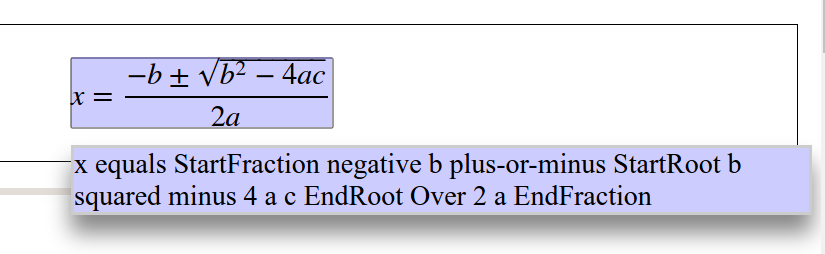
\includegraphics[width=.5\textwidth]{full-equation-cropped.png}
          \hspace{-1.2cm}
          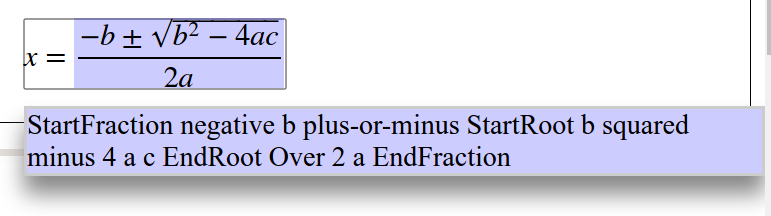
\includegraphics[width=.5\textwidth]{quadratic-step2-cropped.png}
        \item Better support for learning {\LaTeX} via 
          \begin{itemize}
          \item speech rendering of MathJax's informative error messages
          \item voicing of partial expressions and sub-expressions
          \end{itemize}
        \item Abstraction of sub-expressions via responsive equations:
          \hspace*{-1cm}
          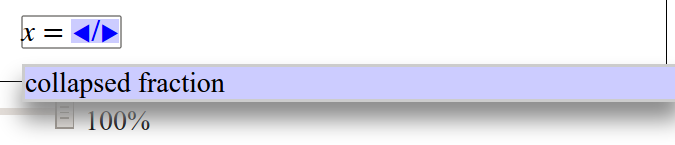
\includegraphics[width=.6\textwidth]{quadratic-step3-cropped.png}
          \hspace{-4cm}
          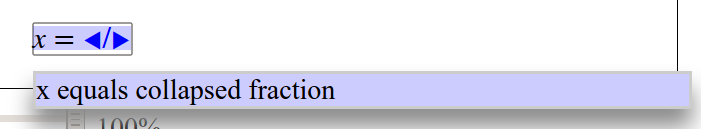
\includegraphics[width=.5\textwidth]{collapsed-quadratic-cropped.png}          
        \end{itemize}
      \end{block}
    \end{column}
    \begin{column}{.32\linewidth}
      \begin{block}{\Large Speech Rule Engine}
        \begin{itemize}
        \item JavaScript library that translates XML expressions into speech
          strings according to rules specified in extended XPath syntax.
        \item Runs both in browsers and as Node module.
        \item Implements a number of features for Maths:
          \begin{itemize}
          \item traditional Mathspeak and ChromeVox's prosody-rich speech rules.
          \item semantic interpretation and enrichment of MathML,
          \item intelligent summaries of sub-expressions,
          \item interactive exploration of expressions, highlighting of DOM
            nodes, etc.
          \end{itemize}
        \item \textcolor{red}{\url{https://github.com/zorkow/speech-rule-engine}}
        \end{itemize}
      \end{block}
      \begin{block}{\Large Supported Activities in Emacs}
        \begin{itemize}
        \item {\LaTeX} editing in AucTeX mode
          \begin{itemize}
          \item Simultaneous visual and aural rendering in AucTeX preview mode.
          \item Integrates with Emacspeak's aural rendering of syntax highlighting
          \end{itemize}
        \item Hydra: Package for temporary or repeatable key bindings
          \begin{itemize}
          \item Voicing and interactive exploration of single {\LaTeX}
            expressions at any time
          \item On key press Maths input via the minibuffer
          \end{itemize}
        \item EWW: Emacs Web Browser
          \begin{itemize}
          \item Alt text given as {\LaTeX} or AsciiMath can be voiced and explored
          \item Examples: Wikipedia, MathWorld
          \end{itemize}
        \item Calc: Emacs Calculator with many symbolic features
          \begin{itemize}
          \item Symbolic expressions can be inserted and output as {\LaTeX}
          \item Last expression can be voiced and explored
          \end{itemize}
        \end{itemize}
        System is available at:\\
        \textcolor{red}{\url{https://github.com/zorkow/emacs-math-speak}}
      \end{block}
    \end{column}
  \end{columns}
\end{frame}
\end{document}

% Motivation
% Solution
% Systems involved:
% Emacsspeak
% Speech Rule Engine
% MathJax Node
% Integration: Node Bridge
% Features
% Other Systems

%%%%%%%%%%%%%%%%%%%%%%%%%%%%%%%%%%%%%%%%%%%%%%%%%%%%%%%%%%%%%%%%%%%%%%%%%%%%%%%%%%%%%%%%%%%%%%%%%%%% 
%%% Local Variables: 
%%% mode: latex
%%% TeX-PDF-mode: t
%%% TeX-master: t
%%% End:
